\documentclass[journal]{IEEEtran}


% correct bad hyphenation here
\hyphenation{op-tical net-works semi-conduc-tor}
\usepackage{amsmath}
\usepackage{comment}
%\usepackage{cases}
%\usepackage{subeqnarray}
\usepackage{booktabs}   %% For formal tables:
                        %% http://ctan.org/pkg/booktabs
\usepackage{subcaption} %% For complex figures with subfigures/subcaptions
                        %% http://ctan.org/pkg/subcaption
\usepackage{xcolor}
\usepackage{listings}
\lstset{
  basicstyle=\fontsize{9}{10}\selectfont\ttfamily,
  numbers=left,
  numberstyle= \tiny,
  keywordstyle= \color{ blue!70},
  commentstyle= \color{red!50!green!50!blue!50},
  frame=single,
  rulesepcolor= \color{ red!20!green!20!blue!20} ,
  escapeinside=``,
  xleftmargin=1.5em,xrightmargin=0em, aboveskip=1em,
  framexleftmargin=2em,
  showstringspaces=false,
  showtabs=false,
  breaklines=true
}
\lstdefinelanguage{Solidity}
{
  morekeywords={contract, mapping, address, uint, private, function, public, if, payable},
  morecomment=[l]{//},
  morestring=[b]"
}


\usepackage{multicol}
\usepackage{lipsum}
\usepackage{mathtools}
\usepackage{cuted}

\usepackage{amsmath}
\usepackage{extpfeil}
\usepackage{mathpartir}
\usepackage[mathscr]{eucal}

\usepackage{hyperref}
\usepackage{cleveref}

\crefformat{section}{\S#2#1#3} % see manual of cleveref, section 8.2.1
\crefformat{subsection}{\S#2#1#3}
\crefformat{subsubsection}{\S#2#1#3}


\begin{document}
%
% paper title
% Titles are generally capitalized except for words such as a, an, and, as,
% at, but, by, for, in, nor, of, on, or, the, to and up, which are usually
% not capitalized unless they are the first or last word of the title.
% Linebreaks \\ can be used within to get better formatting as desired.
% Do not put math or special symbols in the title.
\title{Motion Illusion Detection and Creation}
%
%
% author names and IEEE memberships
% note positions of commas and nonbreaking spaces ( ~ ) LaTeX will not break
% a structure at a ~ so this keeps an author's name from being broken across
% two lines.
% use \thanks{} to gain access to the first footnote area
% a separate \thanks must be used for each paragraph as LaTeX2e's \thanks
% was not built to handle multiple paragraphs
%

\author{
	Shangning~Xu,~\IEEEmembership{SJTU,}
	Jinyu~Li,~\IEEEmembership{SJTU,}
	Zhongye~Wang,~\IEEEmembership{SJTU,}
	Xiaoyi~Bao,~\IEEEmembership{SJTU,}
	and Chenxuan~Li,~\IEEEmembership{SJTU}
}

% The paper headers
\markboth{Journal of \LaTeX\ Class Files,~Vol.~13, No.~9, September~2014}%
{Shell \MakeLowercase{\textit{et al.}}: Bare Demo of IEEEtran.cls for Journals}
% The only time the second header will appear is for the odd numbered pages
% after the title page when using the twoside option.
%
% *** Note that you probably will NOT want to include the author's ***
% *** name in the headers of peer review papers.                   ***
% You can use \ifCLASSOPTIONpeerreview for conditional compilation here if
% you desire.


% make the title area
\maketitle

% As a general rule, do not put math, special symbols or citations
% in the abstract or keywords.
\begin{abstract}
The abstract goes here.
\end{abstract}

% Note that keywords are not normally used for peer review papers.
\begin{IEEEkeywords}
Motion Illusion, Deep Neural Network, Generative Adversary Network
\end{IEEEkeywords}


\IEEEpeerreviewmaketitle


\section{Introduction}
\label{sec:intro}
\IEEEPARstart{M}{otion} illusion is one type of optical illusion where people perceive motions from some static images.
Figure~\ref{fig:motion_example} shows some sample images with illusory motions.
\begin{figure}[h]
	\centering
	\begin{minipage}{0.48\linewidth}
		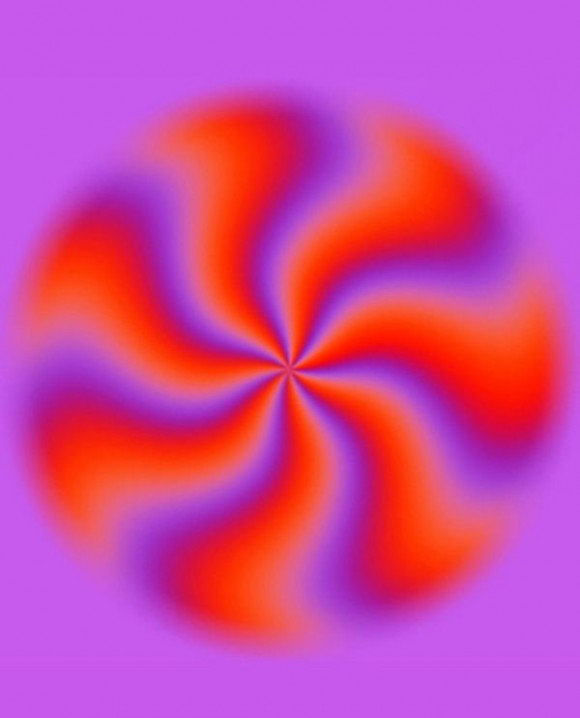
\includegraphics[width=\linewidth]{fig/illusion_eg.jpg}
	\end{minipage}\hfill
	\begin{minipage}{0.48\linewidth}
		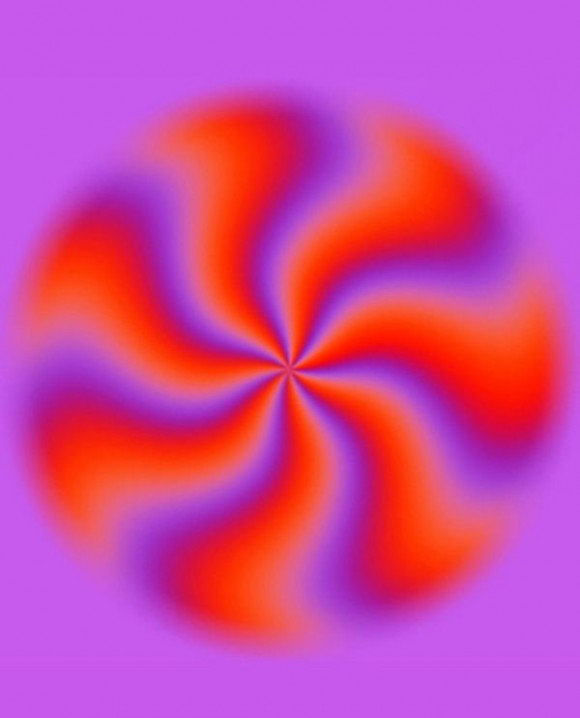
\includegraphics[width=\linewidth]{fig/illusion_eg.jpg}
	\end{minipage}
	\caption{Motion Illusion Examples}
	\label[]{fig:motion_example}
\end{figure}

Rest of the introduction \dots

\section{Motion Illusion Detection: Prednet \& Flownet}
\label{sec:detection}
In this section, we will address the detection problem of motion illusion in static images.
We first explore and re-implement illusion reproduction strategy devised by Watanable \textit{et al.} \cite{watanable2018illusory} in \cref{sec:detection_dnn}, where they use a combination of Prednet \cite{lotter2016deep}, a deep neural network, and optical flow analysis to identify illusory motions.
Based on such strategy, we extract several metrics to evaluate the intensity of illusory motion of images in \cref{sec:detection_measure}.

We embed entire detector into a neural network by implementing the optical flow analysis using the Flownet \cite{ilg2017flownet}.
Therefore, we could easily get back-propagated feedback on how to improve the illusory image.
The integrated detector with Flownet (IDF) serves as a static discriminator in the illusion generative model we propose in \cref{sec:generation}.

\subsection{Detecting Motion Illusion by DNN \& Optic Flow Analysis}
\label{sec:detection_dnn}
Watanable \textit{et al.} \cite{watanable2018illusory} manage to reproduce the illusory motion human perceive from images.
The key idea in their strategy is to simulate the visual perception of human.
Unlike machines, human do not treat the visual input to their eyes as separated images, but instead as a consecutive sequence of image, i.e., a video.
When human observing the image with illusory motions, they tend to believe the image is part of the dynamic video they see through eyes.
In the meantime, the illusion information embedded in images relies on such belief that the image is not static and can produce motions.
Therefore, human can perceive these information, while the computer treat images as numerous static pixels and would neglect those information.

Guided by this intuition, they first use Prednet, a DNN model that predicts future frames in a video given first few frames, to simulate the process of human thinking images as videos.
They then apply the optical flow analysis to the generated video to extract the optical flow vector at some critical pixels.
These vectors can be interpreted as velocity vectors of the illusory motion.
Figure~\ref{fig:scheme} shows the scheme diagram for such reproduction strategy.

\begin{figure}[h]
	\centering
	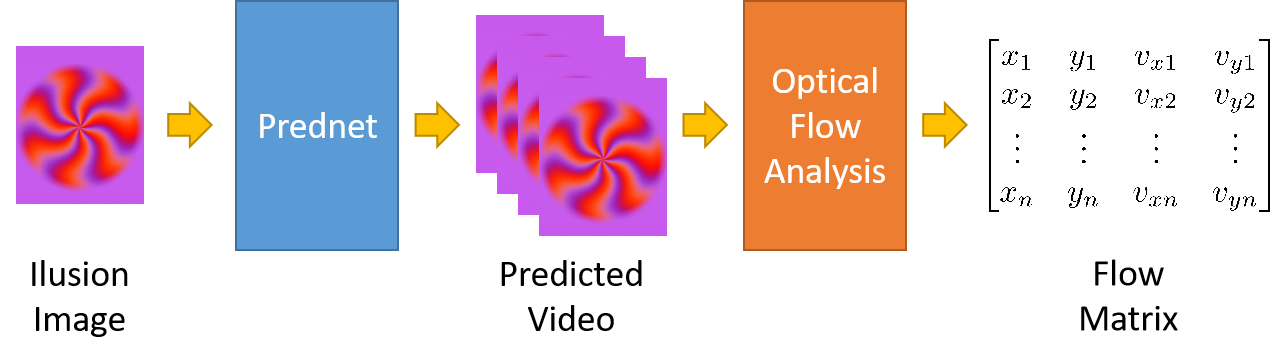
\includegraphics[width=\linewidth]{fig/pred-flow-procedure.png}
	\caption{Prednet-Flow Scheme for Illusion Reproduction}
	\label{fig:scheme}
\end{figure}

% $$
% \left[\begin{matrix}
% 	x_1 & y_1 & v_{x1} & v_{y1} \\
% 	x_2 & y_2 & v_{x2} & v_{y2} \\
% 	\vdots & \vdots & \vdots & \vdots \\
% 	x_n & y_n & v_{xn} & v_{yn} \\
% \end{matrix}\right]
% $$


\subsection{Measuring Illusion Intensity}
\label{sec:detection_measure}

\subsection{Integrated Detector with Flownet}
\label{sec:detection_idf}

\section{Motion Illusion Creation: Asymmetric GAN}
\label{sec:generation}

\subsection{Motion Illusion Generator}
\label{sec:generation_generator}

\subsection{Sanity Constraint Criteria}
\label{sec:generation_criteria}

\section{Experiments}
\label{sec:experiments}

\subsection{Dataset}

Existing collections of illusion images feature variety rather than volume or machine readability, because these images are typically shared on social networks, displayed on websites and consumed by human beings. Robert and Roman's optical illusion image dataset \cite{williams2018optical} could be the first dataset about optical illusion published for research but lacks in organization. In light of these limitations,


%%%%%%%%%%%%%%%%%%%%%%%%%%%%%%%%%%%%%%%%%%%%%%%%%%%%%%%%%%%%%%%%%%%%%%%%%%%%%%%%
% Describe how we collect the images: where are the images from and criteria
%%%%%%%%%%%%%%%%%%%%%%%%%%%%%%%%%%%%%%%%%%%%%%%%%%%%%%%%%%%%%%%%%%%%%%%%%%%%%%%%

\subsection{Results}

We use our own dataset for next-frame prediction and illusion detection. Due to the small size of our dataset, it is feasible for us to evaluate the effectiveness of our detection method on each image, both in the ``rotate'' group and the control group. We predict 22 frames for each image, and then the optical flow between the original image and its 7th frame is computed with Flownet and the traditional Lucas-Kanade method. Some representative images and their results are shown in Fig.~\ref{fig:representative-img-and-results}. For intuitiveness, the optical-flow vector field computed by Flownet is sampled on fixed interval and plotted in Fig.~\ref{fig:vector-fields}.

\subsection{Observations}

From our experiment results in Fig.~\ref{fig:representative-img-and-results} and Fig.~\ref{fig:vector-fields}, some observations can be drawn:

\paragraph{Neural networks can capture the motion in illusion images} From a human perspective, the 7th frame predicted by Prednet in Fig.~\ref{fig:representative-img-and-results} is almost identical to the original image, apart from the brightness change. However, Prednet predicts that the next frames of illusion images will have small motion compared with the original image.

Traditional methods like Lucas-Kanade for computing the optical flow have the disadvantage that they work in a small neighborhood of the image and perform worse for images with significant motion. But in our task, the Lucas-Kanade method better captures the details in the predicted images and thus actually have an advantage.

To further verify our findings, we compute optical flow for all images in our dataset and plot a histogram about magnitudes in Fig.~\ref{fig:histogram-of-magnitudes}. There is a significant difference in the distribution of magnitudes between the control images and the illusion images, which confirms the plausibility of our detection method.

\begin{figure}[t]
  \centering
  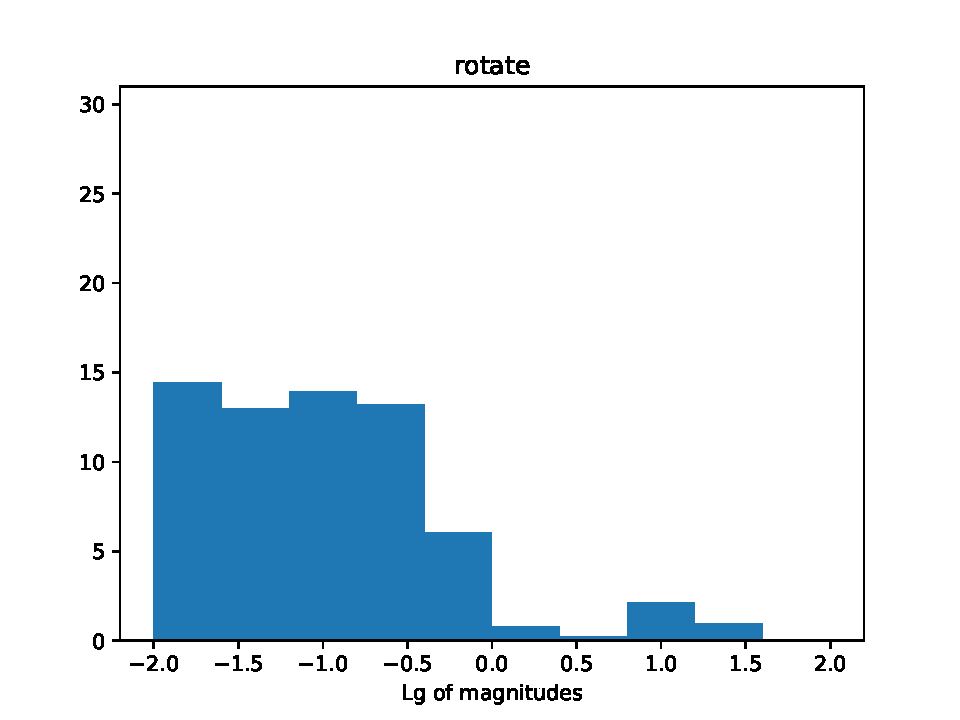
\includegraphics[width=\linewidth]{fig/flow-mag-plot-rotate.pdf}
  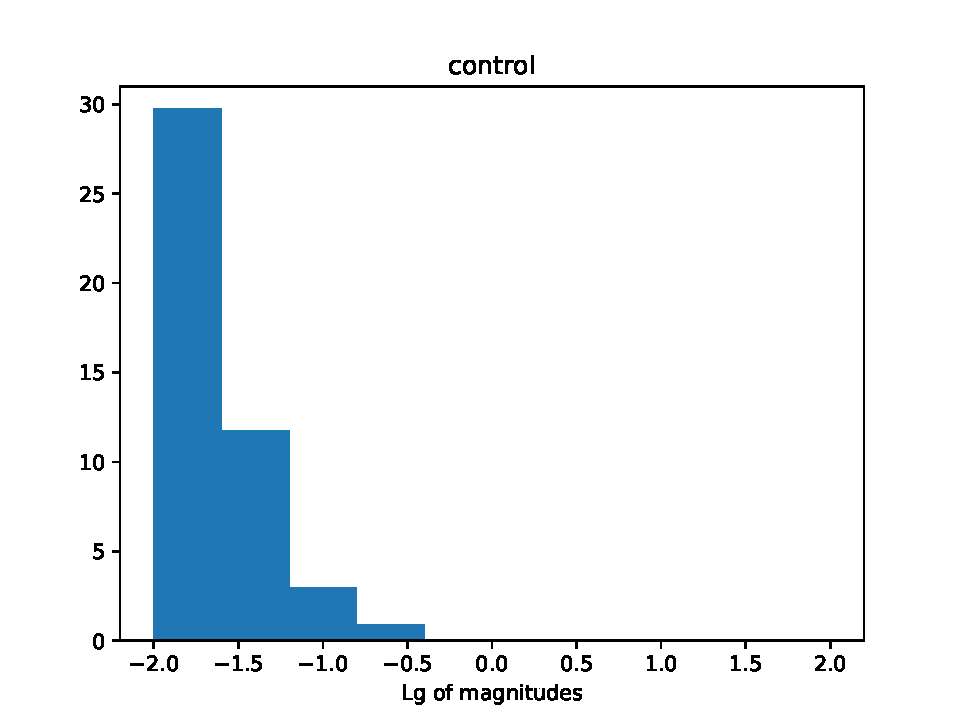
\includegraphics[width=\linewidth]{fig/flow-mag-plot-control.pdf}
  \caption{Histogram of magnitudes of optical-flow vectors computed with the Lucas-Kanade method, for the control and the ``rotate'' group.}
  \label{fig:histogram-of-magnitudes}
\end{figure}

\paragraph{Prednet fails to recognize the direction of illusionary motion} Even though Prednet can ``see'' the illusion in the image, it misses the rotation direction in the illusion images, as evident in the last image of the second column of Fig.~\ref{fig:representative-img-and-results}. Some illusion images have directed rather than rotational motion. These images may be mistakenly classified as images with rotational illusion.

\paragraph{Prednet's prediction seems to be highly dependent on the training dataset} In Watanabe \textit{et al.}'s experiment, Prednet, when trained on videos from the First-Person
Social Interactions Dataset \cite{fathi2012social}, predicts significant and visible rotation for the upper-left image in Fig~.\ref{fig:representative-img-and-results}. But their experiment is limited to one single image and due to hardware limitation, we are unable to verify our hypothesis.

\begin{figure*}
  \centering
  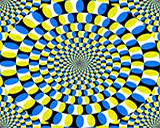
\includegraphics[width=0.24\linewidth]{fig/rotate-0.png}
  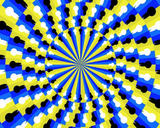
\includegraphics[width=0.24\linewidth]{fig/rotate-1.png}
  
\includegraphics[width=0.24\linewidth]{fig/control-0.png}
  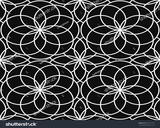
\includegraphics[width=0.24\linewidth]{fig/control-1.png}

  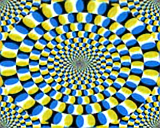
\includegraphics[width=0.24\linewidth]{fig/rotate-0-7.png}
  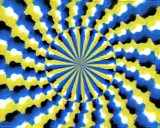
\includegraphics[width=0.24\linewidth]{fig/rotate-1-7.png}
  
\includegraphics[width=0.24\linewidth]{fig/control-0-7.png}
  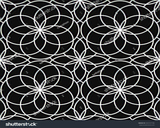
\includegraphics[width=0.24\linewidth]{fig/control-1-7.png}

  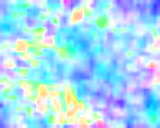
\includegraphics[width=0.24\linewidth]{fig/rotate-0-flo.png}
  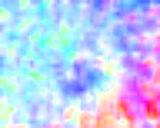
\includegraphics[width=0.24\linewidth]{fig/rotate-1-flo.png}
  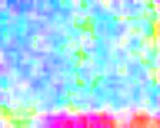
\includegraphics[width=0.24\linewidth]{fig/control-0-flo.png}
  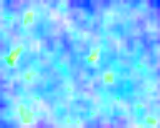
\includegraphics[width=0.24\linewidth]{fig/control-1-flo.png}

  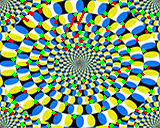
\includegraphics[width=0.24\linewidth]{fig/lk-rotate-0.png}
  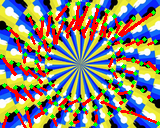
\includegraphics[width=0.24\linewidth]{fig/lk-rotate-1.png}
  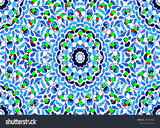
\includegraphics[width=0.24\linewidth]{fig/lk-control-0.png}
  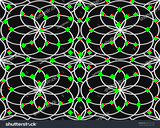
\includegraphics[width=0.24\linewidth]{fig/lk-control-1.png}

  \caption{Some representative images. The first row consists of the original images. The second row is the 7th frame predicted by Prednet from the original image. Optical flows are computed between the original image and the 7th frame. The third row is the optical- flow vector field computed by Flownet and visualized with a color field. Each color represents a direction. Output for the Lucas-Kanade method is optical-flow vectors at keypoints in the images, in the fourth row. In and only in visualization, all optical-flow vectors computed using the Lucas-Kanade are scaled 60 times before drawing for clear comparison.}
  \label{fig:representative-img-and-results}
\end{figure*}

\begin{figure*}
  \centering
  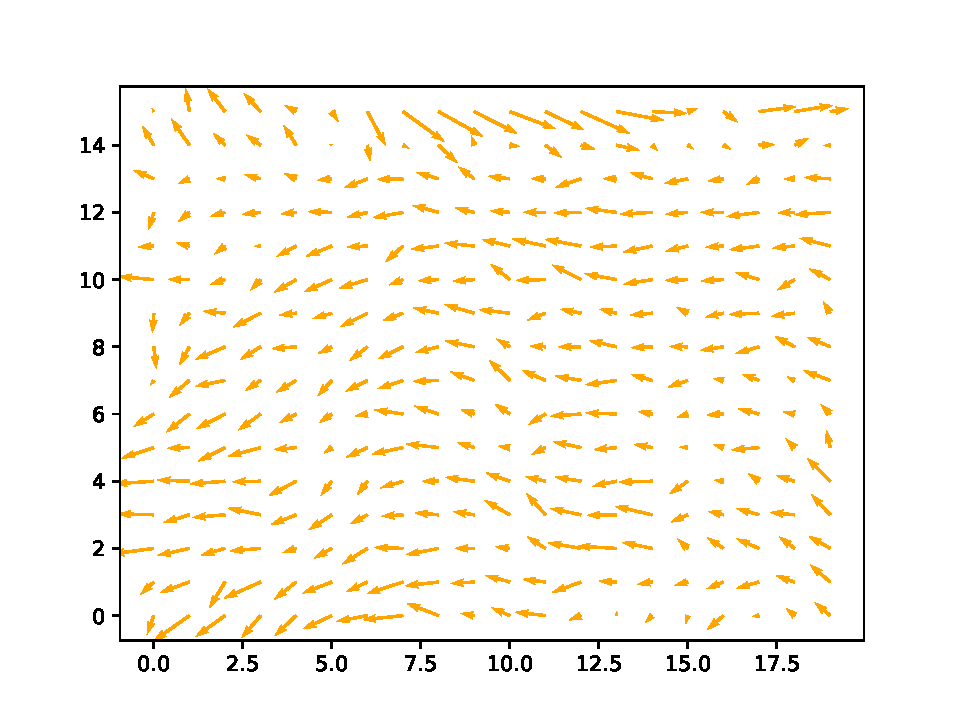
\includegraphics[width=0.45\linewidth]{fig/control-0-vector-field.pdf}
  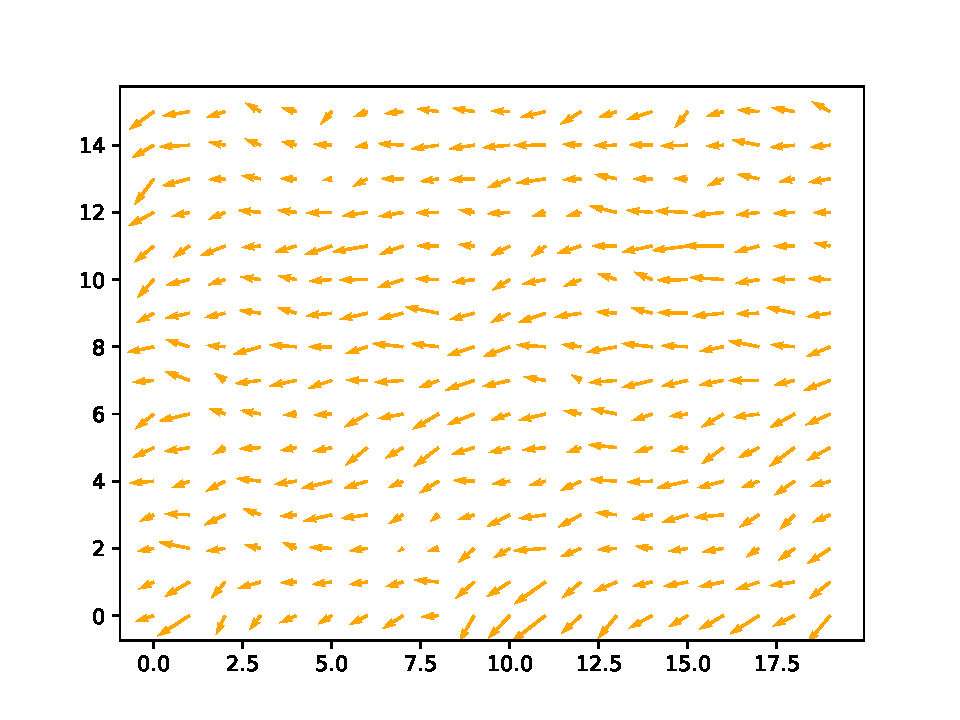
\includegraphics[width=0.45\linewidth]{fig/control-1-vector-field.pdf}

  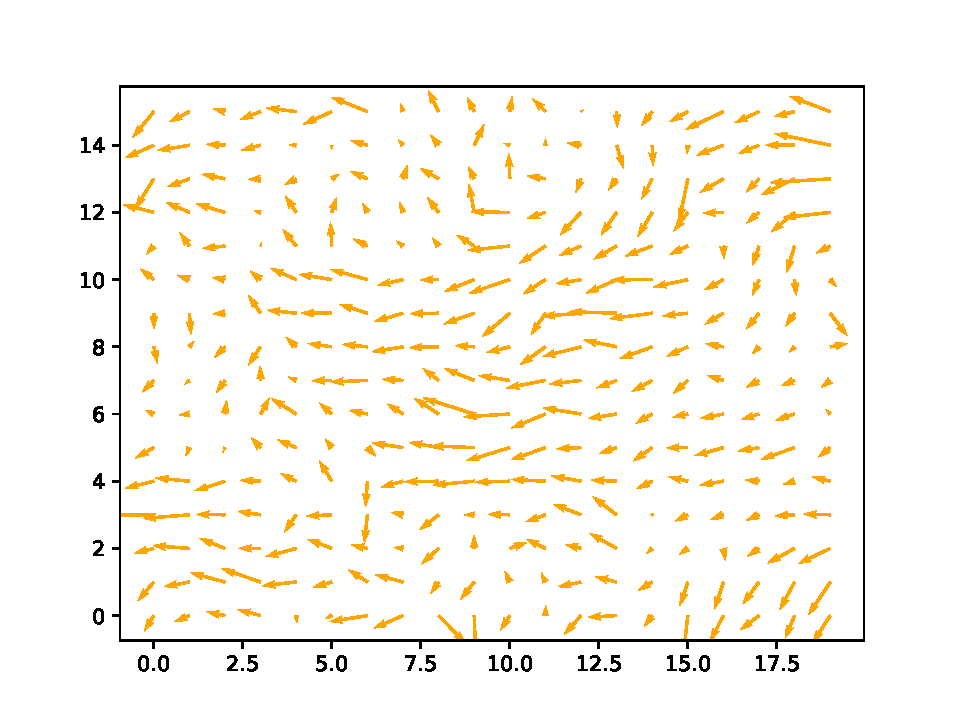
\includegraphics[width=0.45\linewidth]{fig/rotate-0-vector-field.pdf}
  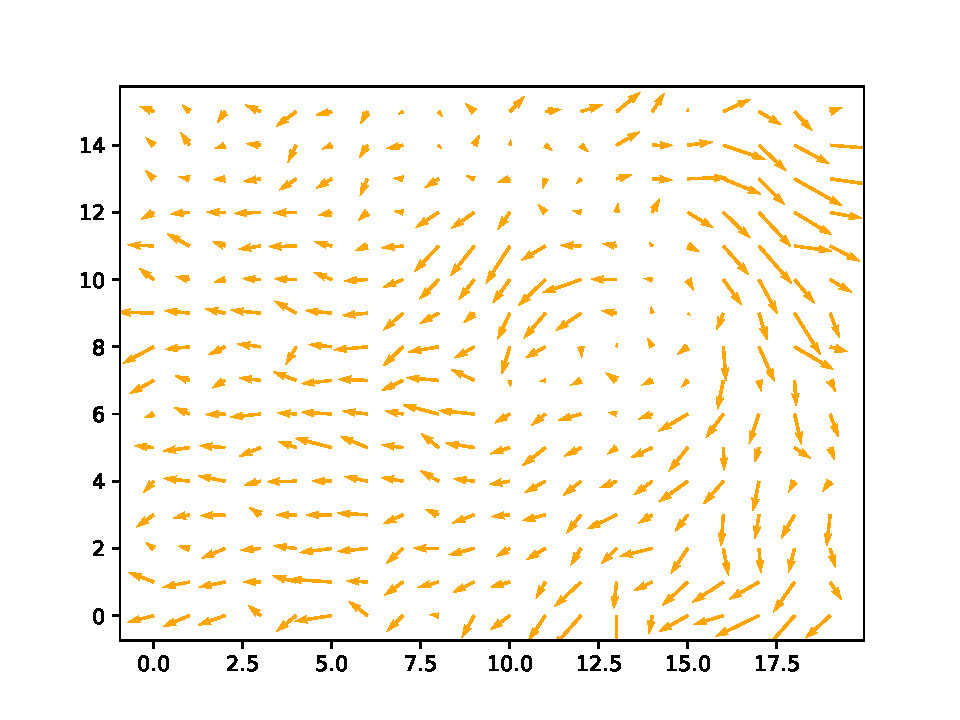
\includegraphics[width=0.45\linewidth]{fig/rotate-1-vector-field.pdf}

  \caption{Plotted optical-flow vector fields computed by Flownet. Each plot from left to right, up to down, corresponds to the images in Fig.~\ref{fig:representative-img-and-results} in a left-to-right order.}
  \label{fig:vector-fields}
\end{figure*}

\section{Related Work}
\label{sec:related}

\section{Conclusion}
\label{sec:conclusion}
The conclusion of the paper \dots



\bibliographystyle{IEEEtran}
\bibliography{ref}

\end{document}
